\documentclass{article}
\usepackage{tikz}
\usetikzlibrary{shapes.geometric, arrows.meta, positioning}

\tikzstyle{startstop} = [rectangle, rounded corners, minimum width=3.5cm, minimum height=1.2cm,text centered, draw=black, fill=blue!20]
\tikzstyle{process} = [rectangle, minimum width=3.5cm, minimum height=1.2cm, text centered, draw=black, fill=orange!20]
\tikzstyle{arrow} = [thick,->,>=stealth]

\begin{document}

\begin{center}
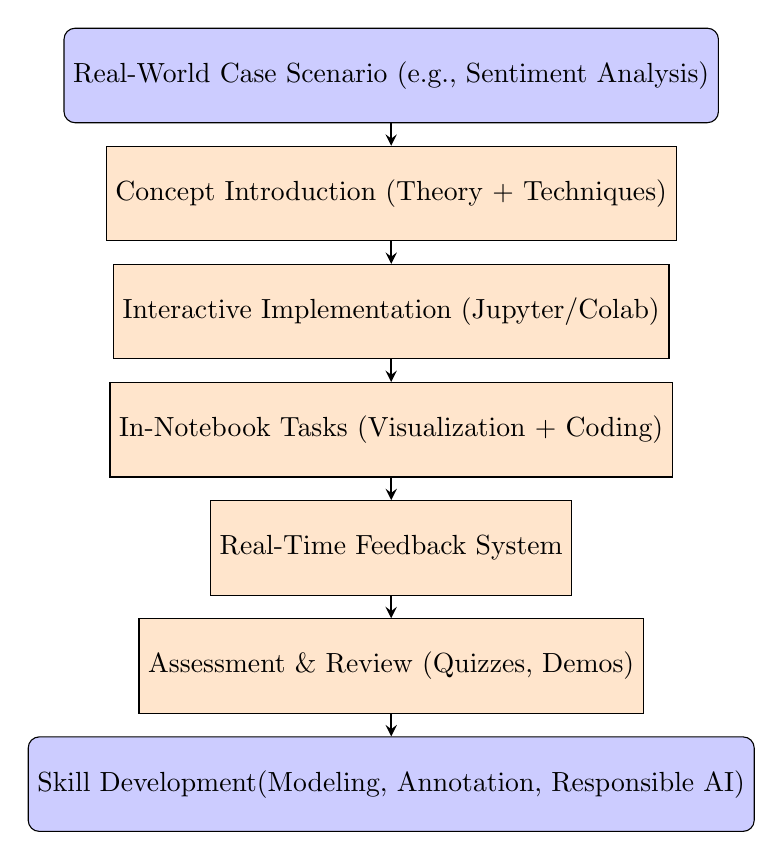
\begin{tikzpicture}[node distance=1.5cm]

% Nodes
\node (start) [startstop] {Real-World Case Scenario (e.g., Sentiment Analysis)};
\node (theory) [process, below of=start] {Concept Introduction (Theory + Techniques)};
\node (impl) [process, below of=theory] {Interactive Implementation (Jupyter/Colab)};
\node (task) [process, below of=impl] {In-Notebook Tasks (Visualization + Coding)};
\node (feedback) [process, below of=task] {Real-Time Feedback System};
\node (assess) [process, below of=feedback] {Assessment \& Review (Quizzes, Demos)};
\node (skill) [startstop, below of=assess] {Skill Development \\ (Modeling, Annotation, Responsible AI)};

% Arrows
\draw [arrow] (start) -- (theory);
\draw [arrow] (theory) -- (impl);
\draw [arrow] (impl) -- (task);
\draw [arrow] (task) -- (feedback);
\draw [arrow] (feedback) -- (assess);
\draw [arrow] (assess) -- (skill);

\end{tikzpicture}
\end{center}

\end{document}
